\documentclass[9pt]{article}

\usepackage[utf8]{inputenc}
\usepackage[T1]{fontenc}

\usepackage[margin=2cm]{geometry}

\newcommand{\noun}[1]{\textsc{#1}}

\usepackage[strict]{changepage}

\usepackage{CJKutf8}
%\begin{CJK*}{UTF8}{zhsong}
%文章内容。
%\clearpage\end{CJK*}
\newcommand{\cn}[1]{
  \begin{CJK*}{UTF8}{gbsn}
  #1
  \end{CJK*}
}

\usepackage{background}

\usepackage{soul}

\backgroundsetup{%
    scale=1.2,
    angle=0,
    contents={%
        \begin{tikzpicture}
            %\pgfmathsetmacro{\myopacity}{mod(\thepage-1,4)*0.25+0.25}
            \node[opacity=0.35] {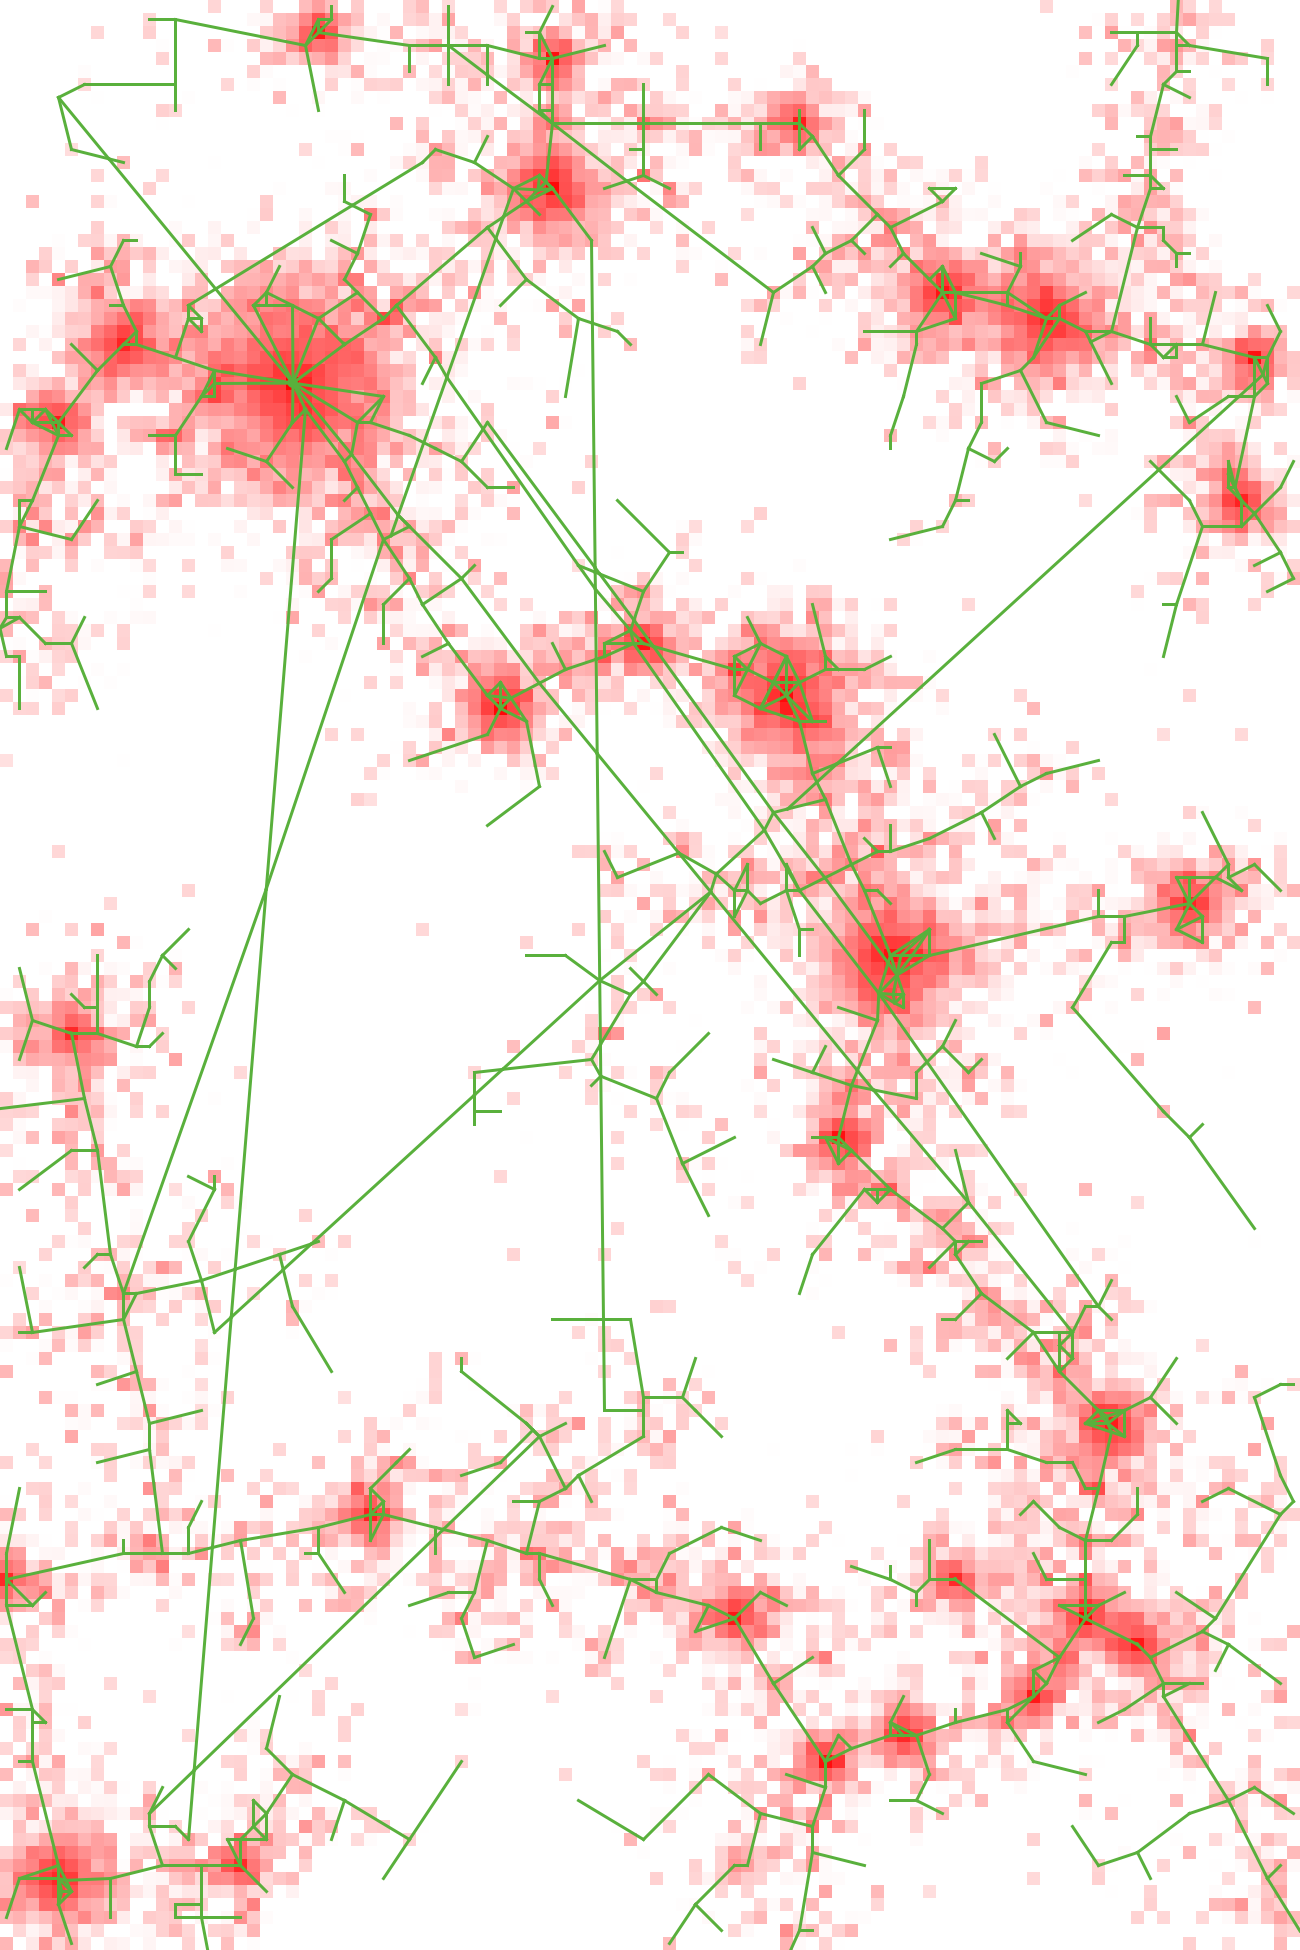
\includegraphics[width=\textwidth]{../Figures/Cover/cover2}};
        \end{tikzpicture}
    }
}




\begin{document}

\pagenumbering{gobble}


\noindent\textbf{Caractérisation et modélisation de la co-évolution des réseaux de transport et des territoires}

\bigskip

\noindent\textbf{Mots-clés : } Territoires ; Réseaux de Transport ; Co-évolution ; Morphogenèse ; Théorie Évolutive des Villes ; Épistémologie Quantitative ; Systèmes de Villes ; Morphologie Urbaine ; Grand Paris ; Delta de la Rivière des Perles

\bigskip

\noindent
L'identification d'effets structurants des infrastructures de transports sur la dynamique des territoires reste un défi scientifique ouvert. Cette question est une des facettes de recherches sur la complexité des dynamiques territoriales, au sein desquelles territoires et réseaux de transport seraient en co-évolution. L'objectif de cette thèse est de mettre à l'épreuve cette vision des interactions entre réseaux et territoires, autant sur le plan conceptuel que sur le plan empirique, en les intégrant au sein de modèles de simulation des systèmes territoriaux. La nature intrinsèquement pluri-disciplinaire de la question nous conduit à mener un travail d'épistémologie quantitative, qui permet de dresser une carte du paysage scientifique et une description des éléments communs et des spécificités des modèles traitant la co-évolution entre réseaux et territoires dans chaque discipline. Nous proposons ensuite une définition de la co-évolution, ainsi qu'une méthode de caractérisation empirique, basée sur une analyse de corrélations spatio-temporelles. Deux pistes complémentaires de modélisation, correspondant à des ontologies et des échelles différentes sont alors explorées. A l'échelle macroscopique, nous construisons une famille de modèles dans la lignée des modèles d'interaction au sein des systèmes de villes développés par la Théorie Evolutive des Villes (Pumain, 1997). Leur exploration montre qu'ils capturent effectivement des dynamiques de co-évolution, et leur calibration sur des données démographiques pour le système de villes français (1830-1999) quantifie l'évolution des processus d'interaction comme l'effet tunnel ou le rôle de la centralité. A l'échelle mésoscopique, un modèle de morphogenèse capture la co-évolution de la forme urbaine et de la topologie du réseau. Il est calibré sur les indicateurs correspondants pour la forme et la topologie locales calculés pour l'ensemble de l'Europe. De multiples processus d'évolution du réseau s'avèrent être complémentaires pour reproduire la grande variété des configurations observées, au niveau des indicateurs ainsi que des interactions entre indicateurs. Ces résultats suggèrent de nouvelles pistes d'exploration des modèles urbains intégrant les dynamiques co-évolutives dans une perspective multi-échelles.

\vspace{1.5cm}

\noindent\textbf{Characterizing and modeling the co-evolution of transportation networks and territories}

\bigskip

\noindent\textbf{Keywords: } Territories; Transportation Networks; Co-evolution; Morphogenesis; Evolutive Urban Theory; Quantitative Epistemology; Systems of Cities; Urban Morphology; Greater Paris; Pearl River Delta

\bigskip

\noindent
The identification of structuring effects of transportation infrastructure on territorial dynamics remains an open research problem. This issue is one of the aspects of approaches on complexity of territorial dynamics, within which territories and networks would be co-evolving. The aim of this thesis is to challenge this view on interactions between networks and territories, both at the conceptual and empirical level, by integrating them in simulation models of territorial systems. The intrinsically multidisciplinary nature of the question requires first to proceed to a quantitative epistemology analysis, that allow us to draw a map of the scientific landscape and to give a description of common features and specificities of models studying the co-evolution between network and territories within each discipline. We propose consequently a definition of co-evolution and an empirical method for its characterization, based on spatio-temporal correlation analysis. Two complementary modeling approaches, that correspond to different scales and ontologies, are then explored. At the macroscopic scale, we build a family of models inheriting from interaction models within system of cities, developed by the Evolutive Urban Theory (Pumain, 1997). Their exploration shows that they effectively capture co-evolutionary dynamics, and their calibration on demographic data for the French system of cities (1830-1999) quantifies the evolution of interaction processes such as the tunnel effect or the role of centrality. At the mesoscopic scale, a morphogenesis model captures the co-evolution of the urban form and of network topology. It is calibrated on corresponding indicators for local form and topology, computed for all Europe. Multiple network evolution processes are shown complementary to reproduce the large variety of observed configurations, at the level of indicators but also interactions between indicators. These results suggest new research directions for urban models integrating co-evolutive dynamics in a multi-scale perspective.



\end{document}

\bigskip


\noindent\cn{\textbf{建模交通网络和地域的共同演变}}

\smallskip

\noindent\cn{\textbf{关键字 : }} \cn{地域; 交通网络; 共同演变; 形态; 演变城市理论; 量化认识论; 城市系统; 城市形态; 大巴黎; 珠江三角洲}

\smallskip

\noindent\cn{运输基础设施对领土体系结构效应存在的问题远未得到解决。% La question de l'existence d'effets structurants des infrastructures de transports sur les systèmes territoriaux est loin d'être résolue. 
这是复杂的地域动态的一个方面,其中领土和交通网络正在共同演变。% C'est l'une des facettes de dynamiques territoriales complexes, au sein desquelles territoires et réseaux de transport sont en co-évolution.
这篇论文的目的是测试网络和地域之间的相互作用。%L'objectif de cette thèse est de mettre à l'épreuve cette vision des interactions entre réseaux et territoires.
它将在概念和经验上做到这一点,目的是将其整合到地域系统的模拟模型中。% Elle le fera autant sur le plan conceptuel que le plan empirique, dans le but de l'intégrer au sein de modèles de simulation des systèmes territoriaux.
我们正在处理的问题本质上是多学科的。% La problématique que nous traitons est intrinsèquement multi-disciplinaire.
出于这个原因,我们首先进行量化的认识论分析。% Pour cette raison, nous procédons dans un premier temps à une analyse d'épistémologie quantitative. 
它可以绘制科学的景观图,并精确地描述每个学科不同模型的结构。% Elle permet de dresser une carte du paysage scientifique et une description précise de la structure des différents modèles dans chaque discipline.
我们制定了一个共同进化的定义,并开发了一个基于时空相关分析的经验表征方法。% Nous élaborons une définition de la co-évolution et élaborons une méthode de caractérisation empirique basée sur une analyse de correlations spatio-temporelles.
探索两个互补的建模轨道。 它们对应于不同的本体和尺度。% Deux pistes complémentaires de modélisation sont explorées. Elles correspondent à des ontologies et des échelles différentes.
在宏观层面上,我们根据城市演变理论发展起来的城市体系内的相互作用模型发展了一个模型家族。% A l'échelle macroscopique, nous développons une famille de modèles dans la lignée des modèles d'interaction au sein des systèmes de villes développés par la Théorie Evolutive des Villes.
他们的探索表明,他们实际上捕捉到共同演化的动力。 他们对法国城市系统(1830-1999)的人口统计数据的校准量化了互动过程的演变。 这些例如是隧道效应或网络中心性的影响。% Leur exploration montre qu'ils capturent effectivement des dynamiques de co-évolution. Leur calibration sur données démographiques pour le système de villes français (1830-1999) quantifie l'évolution de processus d'interaction. Ceux-ci sont par exemple l'effet tunnel ou l'impact de la centralité dans le réseau.
在介观尺度上,形态演化模型捕捉城市形态和网络拓扑的共同演化。% A l'échelle mesoscopique, un modèle d'évolution morphologique capture la co-évolution de la forme urbaine et de la topologie du réseau.
根据整个欧洲计算的局部形态和拓扑结构的相应指标进行校准。% Il est calibré sur les indicateurs correspondants pour la forme et la topologie locales calculés pour l'ensemble de l'Europe.
网络演进的多个过程被考虑到:成本效益计划,潜在的突破,自组织。 它们似乎是互补的,可以产生所有的真实配置。% De multiples processus d'évolution du réseau sont pris en compte : planification coût-bénéfices, rupture de potentiel, auto-organisation. Ils apparaissent complémentaires pour produire l'ensemble des configurations réelles. 
校准也是按照第二顺序进行的,也就是指标之间的相互作用,模型重现了现有情况的多样性。% La calibration est également faite au second ordre, c'est-à-dire sur les interactions entre indicateurs, pour lequel le modèle reproduit une grande diversité de situations existantes.
这些结果一方面表明了把城市演变理论与形式演变相结合的理论建构。 另一方面,他们开辟了新一代城市模式的探索,这些模型将不得不整合多尺度协同进化动力学。% Ces résultats suggèrent d'une part une construction théorique intégrant Théorie Evolutive Urbaine et évolution de la forme. Ils ouvrent d'autre part l'exploration d'une nouvelle génération de modèles urbains qui devra intègre les dynamiques co-évolutives multi-échelles.
}








%%%%%%%%%%%%%%%%%%%%
%% Biblio
%%%%%%%%%%%%%%%%%%%%


%\begin{multicols}{2}

%\setstretch{0.3}
%\setlength{\parskip}{-0.4em}


%\bibliographystyle{apalike}
%\bibliography{/Users/Juste/Documents/ComplexSystems/CityNetwork/Biblio/Bibtex/CityNetwork}

%\end{multicols}

\end{document}
